\documentclass{article}

\usepackage[backend=biber, style=authoryear, url=false, natbib=true]{biblatex}
\addbibresource{library.bib}
\usepackage[utf8]{inputenc}
\usepackage[T1]{fontenc}
\usepackage[french]{babel}
\usepackage{amsmath,amsfonts,amssymb}
\usepackage{color}
\usepackage{graphicx}
\graphicspath{{./img/}}
\usepackage{url}
\usepackage[lined,boxed,commentsnumbered]{algorithm2e}
\usepackage[french]{cleveref}

\newcommand{\transp}[1]{#1^{\!\top}\!}
\DeclareMathOperator*{\argmax}{arg\,max}

\title{TP5: Réseaux récurrents}
\author{Gaétan Marceau Caron}
\date{\today}

\begin{document}

\maketitle

\section{Introduction}
Lors des séances précédentes, nous nous sommes intéressés à la tâche de la classification d'images avec un réseau neuronal classique.
En particulier, nous n'avons pas pris en compte la topologie naturelle de l'image.
Un réseau de convolution utilise directement cette information en parcourant l'image avec des noyaux qui traitent chaque pixel et son voisinage.
En conséquence, cette information permet au réseau de convolution de dépasser significativement les réseaux classiques dans le traitement d'images.

De manière analogique, différent modèles issus des réseaux de neurones sont adaptés aux structures naturelles des données.
Un exemple important consiste à modéliser la probabilité d'observer une séquence de symboles.
De manière générale, les symboles ne sont pas tous mutuellement indépendants.
Par exemple, dans les langages naturels, la probabilité d'une lettre dépend des lettres voisines.

Les réseaux récurrents sont des réseaux de neurones avec une mémoire permettant d'apprendre un contexte et de faire une prédiction.
Ces réseaux sont adaptés pour l'apprentissage de séquences, c'est-à-dire de données possédant un ordre naturel.
Par exemple, le texte, la vidéo ou l'enregistrement audio sont des séquences pouvant être traitées par des réseaux récurrents.\footnote{voir \url{http://www.hexahedria.com/2015/08/03/composing-music-with-recurrent-neural-networks/}}
Le but du réseau récurrent est alors de prédire la prochaine donnée en apprenant un modèle stochastique.
De plus, une fois entraîné, le réseau peut être utilisé comme modèle génératif.

Dans ce TP5, nous allons étudier un réseau récurrent simple pour la tâche de prédiction de caractères.
Le modèle du langage que nous allons utiliser se définit comme:
\begin{equation}
p(x^1, \dots, x^n) = \prod_{i=1}^n p(x^i|x^1,\dots,x^{i-1}) \quad \mbox{(règle de chaînage)}
\end{equation}
et nous allons modéliser cette loi de probabilité à l'aide d'un réseau récurrent.

\begin{figure}[ht!]
\centering
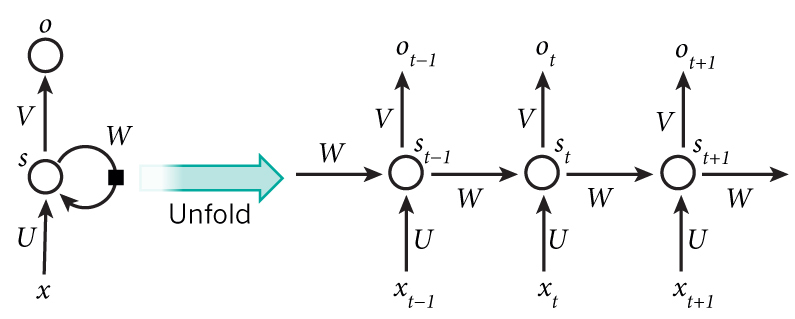
\includegraphics[scale=0.35]{rnn.jpg}
\caption{Déroulement du réseau récurrent ($s=h, U=W_{xh}, V=W_{hy}, W=W_{hh}$)\label{fig:rnn} (source: http://www.wildml.com)}
\end{figure}

Le but du réseau récurrent est de prédire le prochain caractère $o^t$ en fonction des caractères observés $(x^1, \dots, x^{t})$.
Pour modéliser les dépendances à long terme, le réseau est doté d'une mémoire interne $h$ qui est modifiée au cours du temps (nous noterons ces valeurs $h^t$).
Nous pouvons donc définir les équations de la procédure \texttt{forward} permettant de transformer les données en entrée:
\begin{align}
  h_t &= \sigma(W_{xh} x_t + W_{hh} h_{t-1} + b_h) \label{forward1}\\ 
  y_t &= W_{hy} h_{t} + b_y \label{forward2}\\
  p_t &= \mbox{softmax}(y_t) \\
  o_t &\sim p_{t}
\end{align}
où $\sigma$ est une fonction d'activation, $W_{xh}$ est une matrice transformant les entrées en élément de la mémoire, $W_{hh}$ est une matrice carrée propageant la mémoire du temps $t-1$ au temps $t$ et $W_{hy}$ est une matrice qui convertit la mémoire en sortie. De plus, nous utilisons une variable $y^t$ pour les sorties non normalisées et $p^t$ pour les sorties normalisées (la loi de probabilité apprise).
Finalement, nous rappelons, sous la forme d'un pseudocode (cf. algorithme \ref{bptt}), l'algorithme «Backpropation Through Time» (BPTT).

\begin{algorithm}[h]
  \SetAlgoLined
  \KwData{$(x^t,h^t,p^t)_{t=1}^n$}
  \KwResult{$\delta W_{xh}, \delta W_{hh}, \delta W_{hy}, \delta b_{h}, \delta b_{y}$}
  $\delta W_{xh} = 0, \delta W_{hh} = 0, \delta W_{hy} = 0, \delta b_{h} = 0, \delta b_{y} = 0, \delta h^{next} = 0$\;
  \For{t=n to 0}{
    $\delta y = p^t - e_{x^{t+1}}$ \;
    $\delta W_{hy} = \delta W_{hy} + \delta y \cdot \transp{(h^t)}$\;
    $\delta b_y = \delta b_y + \delta y$\;
    $\delta h = \transp{W_{hy}} \cdot \delta y + \delta h^{next}$\;
    $\delta h_{raw} = (1 - h^t \odot h^t) \odot \delta h$\;
    $\delta b_h = \delta b_h + \delta h_{raw}$\;
    $\delta W_{xh} = \delta W_{xh} + \delta h_{raw} \cdot \transp{(x^t)}$\;
    $\delta W_{hh} = \delta W_{hh} + \delta h_{raw} \cdot \transp{(h^{t-1})}$\;
    $\delta h^{next} = \transp{W_{hh}} \cdot \delta h_{raw}$\;
  }
  \caption{Pseudocode de BPTT \label{bptt}}
\end{algorithm}

\section{Description}
Pour ce TP, vous devez compléter le code fourni:
\begin{enumerate}
\item dans la procédure forward (\texttt{model.py::98-99}), implémenter la définition des équations \ref{forward1} et \ref{forward2}
\item dans la procédure backward (\texttt{model.py:110-119}), implémenter l'algorithme BPTT (voir pseudocode \ref{bptt})
\end{enumerate}
Vous pouvez vérifier votre implémentation avec le test des différences finies \texttt{gradCheck:model.py:183}.
Une fois l'implémentation vérifiée, vous pouvez commenter l'appel à \texttt{gradCheck} et admirer les premiers balbutiements de votre réseau récurrent!

\section{Livrable}
\noindent {\bf Date du livrable:} avant le 29 janvier 2016 \newline
{\bf Format du livrable:} un fichier compressé nommé {\it DL\_tp5\_prénom\_nom.zip} contenant le code et le résumé \newline
{\bf Dépôt:} à l'adresse \url{gaetan.marceau-caron@inria.fr} avec comme objet du message {\it DL\_tp5\_prénom\_nom}.\newline
{\bf Description:}\newline
Le livrable associé au TP5 doit contenir le code complété et accompagné d'un résumé de 2 pages maximum.
Le code doit s'exécuter avec la commande \texttt{python model.py} et afficher l'évolution de l'apprentissage (sortie par défaut du programme).
Vous devez décrire l'impact de chaque paramètre du programme sur l'apprentissage (et les phrases générées automatiquement) et aussi proposer une façon d'améliorer le modèle du langage.

\printbibliography

\end{document}
